\documentclass[10pt, logo, copyright, anonymous]{nvidiaextabstract}

\venue{From Human Videos to Dexterous Robot Capability (CoRL 2026)}
\submissionID{Anonymous submission}
\title{Video-Measured Meshes and Static Poses}
\shorttitle{Video-Measured Meshes and Static Poses}

\begin{abstract}
\textbf{Abstract:}
We build meshes and static-object poses from video. Two-fold leave-objects-out
parameter selection gives object Chamfer distance (CD-O) of 0.926\,cm versus
1.008\,cm for boxes and 2.523\,cm for cubes. These estimates reuse ten public
scans. Depth uses MoGe-2 pseudo-labels, not measured depth. Stereo-derived
shrinkage lowers public-train pose errors, but controls show no measurable
calibration benefit over global shrinkage. The gains are consistent with
shrinking wrongly directed offsets; static rollouts do not demonstrate manipulation.
\end{abstract}

\setlength{\textfloatsep}{10pt plus 2pt minus 2pt}
\begin{document}
\raggedbottom
\maketitle

\section{A fixed rule-selection protocol}
Track 3 scores meshes and policy-rollout poses separately~\cite{challenge}.
We fix three categories (vessels, blocks, tools) and two five-object folds.
Video determines shape. Parameters selected on one fold are scored on the other;
then folds swap. Adoption requires mean gain over boxes $>0.03$\,cm, worst
regression $\leq0.15$\,cm, and no pair-mean regression. Cylinders (R1) and
handles (R2) pass; R2 wins. Tool heads (R3) fail the gain gate.

CD-O removes scale and placement under the kit's triangle budget~\cite{challenge}.
Public scans provide scoring references, never submitted geometry, dimensions
or templates~\cite{faq}.

\begin{figure}[t]
\centering
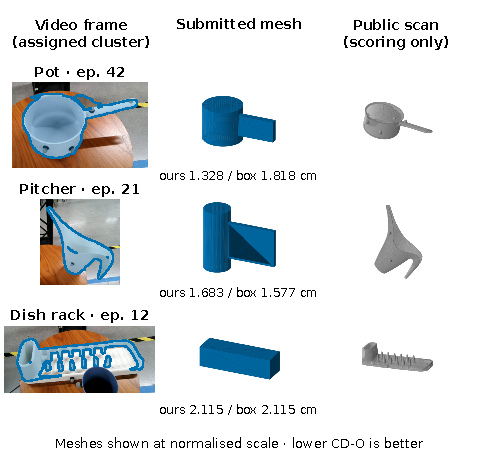
\includegraphics[width=\columnwidth]{figures/d1-v2-qualitative.pdf}
\caption{Video clusters, fitted R2 meshes and public scans at normalized
scale. Rotations are display-only. Labels give three-seed fitted R2 / box CD-O (cm,
$\downarrow$), not cross-fitted scores. Vessel interiors and rack tines are absent.}
\label{fig:qualitative}
\end{figure}

\section{Video measurements}
MoGe-2~\cite{moge2} supplies above-table clusters. We name them manually and
omit merged/clipped objects. Normalized extents remove scale, not distortion;
medians pool frames then episodes. R2 adds thresholded handles or keeps boxes.
Parts retain internal faces.

\section{Results and disclosure}
Cross-fitting uses three sampling seeds (Table~\ref{tab:cdo}).

\begin{table}[t]
\centering
\small
\begin{tabular}{lrr}
\toprule
Mesh & Object mean & Pair mean \\
\midrule
Cube (reused) & 2.523 & 2.772 \\
Box packed v1 & 1.0091 & 1.2547 \\
R2 cross-fitted & \textbf{0.926} & \textbf{1.087} \\
R2 packed v2 & 0.9257 & 1.0850 \\
\bottomrule
\end{tabular}
\caption{CD-O (cm, $\downarrow$), ten public scans. Packed rows use exact
per-pair kit seeds on 26/36 pairs; the spoon is unscanned. Cube and cross-fitted
pair means are reused-object estimates.}
\label{tab:cdo}
\end{table}

R2's worst cross-fitted regression is 0.106\,cm (pitcher). Mean gain is
0.082\,cm over ten objects (sample standard deviation 0.180; standard error
0.057). Threshold means span about 0.002\,cm; the final threshold is 1.30.
Selection chiefly favors R2 over R1; bias remains.

\textbf{Disclosure.} Public scans informed box/ellipsoid selection and episode
39's measurement thresholds. We designed rules after a pot box lost to a cube.
Families, folds and gates preceded new scoring but reuse these ten scans;
cross-fitting is not an untouched test. The unscanned spoon keeps its box
(10/36 pairs, excluded from both means). Sampling seeds cannot measure
new-object uncertainty.

\section{Static-object poses}
FlashCHORD~\cite{flashchord} simulates video-sized boxes with parked hands.
Slots 0/1 mean the first/second roster objects. Aligning slot 0's first pose
rotates slot 1's offset; camera-to-mocap heading is unavailable.

Public train motion-capture (mocap) references support diagnostics. v1 uses video centroids or
defaults. Merged-cluster stacking (K1a) puts an object without its own frame-0
cluster atop the other at the merged centroid. Oracle static fixes reference
first poses for diagnosis only. Unscaled v1/K1a earn no slot-1 AUC credit.
Leave-one-episode-out body-up calibration gave no gain and is unused.

\begin{table}[t]
\centering
\small
\setlength{\tabcolsep}{3pt}
\begin{tabular}{lrrrr}
\toprule
Placement & AUC $\uparrow$ & SP-SR $\uparrow$ & RPE & MPPE \\
\midrule
\multicolumn{5}{l}{Eight train episodes (equal-episode means)} \\
v2 rule & 0.2688 & 0 & 39.36 & 22.82 \\
+ stereo scale (S1) & 0.2690 & 0 & 35.34 & 20.84 \\
Global shrink (G) & 0.2690 & 0 & 35.28 & 20.80 \\
Zero offset (C0) & 0.2748 & 0 & 19.54 & 14.13 \\
\bottomrule
\end{tabular}
\caption{Eight public train episodes. AUC: area under surface-point accuracy curve.
SP-SR: success at mean errors $\leq$10\,cm/0.5\,rad; MP-SR: all-object success at
$<$3\,cm/30$^\circ$ (always zero). RPE: relative-position error; MPPE: six attached
points' mean error (both cm, $\downarrow$).}
\label{tab:pose}
\end{table}

\begin{figure}[t]
\centering
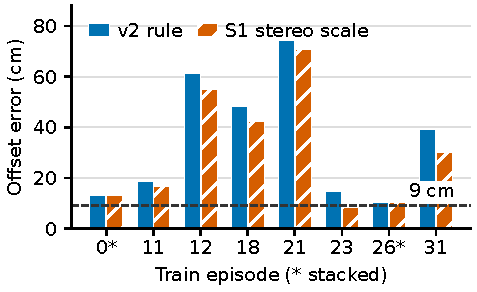
\includegraphics[width=\columnwidth]{figures/d2-slot1-offset.pdf}
\caption{Frame-0 slot-1 (second object) offset error in the first object's
body frame, eight public train episodes. v2 stacks 0/26 (*); S1 stereo-scales
table-plane offsets and is a no-op there. Dashed: 9\,cm, the kit's largest
surface-point AUC threshold~\cite{challenge}, not a trajectory success bound.}
\label{fig:offset}
\end{figure}

The original placement gates failed. \emph{Post-result Amendment 2} added
public episodes 2/27 for confirmation; only 2 was measurable because 27 has
separate clusters. Train episode 26 had already informed selection for its
scored analogue, 28. \emph{Post-result Amendment 3} replaced the all-scene gate
with per-scene checks. Episodes 1/28 passed (\mbox{intended-pose} error 0.062\,cm,
drift 0.058\,cm). Episode 30 kept v1 after its sweeper fell 17\,cm.
Thus v2 stacks train 0/26 only and uses v1 elsewhere.

\textbf{Stereo-derived shrinkage (S1).} Calibrated C/B stereo uses semi-global
block matching (75.47\,mm baseline). S1 shrinks slot 1's table-plane offset by
the median stereo/MoGe-2 ratio, $s=0.819$--0.923, an unvalidated estimate.
Heights, rotations and sizes stay fixed. Train mocap ratios motivated S1.
Selection uses training episodes because tuning 39/42 each have one object.
Estimator and gates preceded scoring. Adoption was \emph{post-result}: we
accepted S1 after it passed the invariance check exactly. Whole-scene scaling
(S2) failed that check due to numerical roundoff. The original global failure
rule would have kept v2; we applied the check to each candidate separately.

Registered controls show no measurable calibration benefit over global shrink
(G, $c=0.857$), which gives MPPE 20.80\,cm versus S1's 20.84.
The gain is consistent with shrinking wrongly directed offsets: zero offset
(C0) gives 14.13\,cm but overlaps boxes. A pre-registered clearance-limited follow-up gives 17.02\,cm but fails AUC
($-0.00018$) and episode-31 MPPE ($+0.69$\,cm $>0.5$) gates; v3 therefore
retains S1, which passed its own fixed gates.

Direction errors remain about 2--130$^\circ$. Residual ratios are 1.18--2.23
(default-offset 31: 3.58). Length-only oracle AUC is 0.2767 versus 0.2688.
Evaluation lacks calibration; public calibration is assumed.

S1 passes physical checks on 13 scenes (intended-pose error $\leq$0.049\,cm, drift $\leq$0.048\,cm).
v2 remains on stacked 1/28, single-object 35--38, and 5 (nonfinite optimizer
state: failed check, cause uninvestigated, no retry). Scored $s=0.768$--0.948.
Diagnostics approximate host vertices with scan surface samples; no host-score
gain is claimed. Missing
concavities, manual identities, frame uncertainty and the unmeasured spoon
limit generality.

\begin{figure}[htbp]
\centering
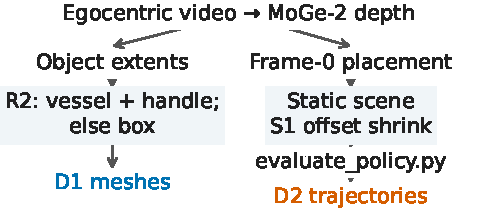
\includegraphics[width=\columnwidth]{figures/pipeline.pdf}
\caption{S1's calibration benefit is unproven; failed physical checks retain v2.}
\label{fig:pipeline}
\end{figure}

\typeout{TRACK3-MAIN-TEXT-END-PAGE: \thepage}
\typeout{TRACK3-TABLE-PAGE: \getpagerefnumber{tab:cdo}}
\typeout{TRACK3-FIGURE-PAGE: \getpagerefnumber{fig:qualitative}}
\typeout{TRACK3-POSE-TABLE-PAGE: \getpagerefnumber{tab:pose}}
\typeout{TRACK3-PIPELINE-FIGURE-PAGE: \getpagerefnumber{fig:pipeline}}
\typeout{TRACK3-OFFSET-FIGURE-PAGE: \getpagerefnumber{fig:offset}}
\clearpage
\bibliographystyle{plainnat}
\bibliography{references}
\end{document}
